\section{Navigation}
\label{test:navigation}
The robot must visit a set of waypoints while avoiding obstacles on its path and finally following a person outside the arena.

\subsection{Focus}
This test focuses on tracking and recognizing a previously unknown person, obstacle avoidance, obstacle interaction, and safe navigation in dynamic environments in general.

\subsection{Setup}

\begin{enumerate}
	\item \textbf{Doors:} All doors in the apartment are open, except for the entry door. 
	\item \textbf{Location:} One of the arenas (apartment) and its surroundings. The apartment is in its normal state. Part of the test is performed outside the arena in a public space.
	The arena will likely contain another door that may be used for this test.
	\item \textbf{Operator:} A \quotes{professional} operator is selected by the TC to test the robot during the guiding phases.
	\item \textbf{Other people:} There are no restrictions on other people walking by or standing around throughout the complete task.
	\item \textbf{Path:} A path is setup beforehand and announced, except for Waypoint 4 (later explained).
\end{enumerate}

\subsection{Task}
%%%%%%%%%%%%%%%%%%%%%%%%%%%%%%%%%%%%%%%%%%%%%%%%%%%%%%%%%%%%%%%%%%%%%%
%
% Redundant text. Lets keep it simple. [Mauricio Matamoros]
%
%%%%%%%%%%%%%%%%%%%%%%%%%%%%%%%%%%%%%%%%%%%%%%%%%%%%%%%%%%%%%%%%%%%%%%
% The robot must visit a set of waypoints (rooms, placement locations, furniture, beacons, landmarks, etc.) while avoiding the obstacles on its path. Unless stated otherwise, waypoints may be on the floor. The robot must state when it reached a new waypoint or is not able to reach a waypoint. At the last waypoint inside the arena, the robot must follow a human which will lead the robot outside. After the robot is commanded to stop following, the robot must guide a (different) human back to the apartment.

\begin{enumerate}
	\item \textbf{Entering:} The robot enters the arena.

	\item \textbf{Waypoint 1 (path planning):} After entering the arena, the robot must navigate to \textit{Waypoint 1} that is reachable via, at least, two paths, each one requiring the robot to go through a door which will be shut as the robot approaches. The robot may:
	\begin{itemize}
		\item Take a different path.
		\item Open the closed internal door.
	\end{itemize}

	\item \textbf{Waypoint 2 (obstacle interaction):} Immediately after reaching \textit{Waypoint 1}, the robot must go to and reach at grasp (or place) distance \textit{Waypoint 2}, a placement location (e.g. a shelf). A large obstacle will prevent the robot from getting close to its destination, having the robot to identify it and interact with it.
	Possible actions include:
	\begin{itemize}
		\item Gently move the obstacle (e.g.~if the obstacle is an object).
		\item Gently ask the obstacle to move away (e.g.~if the obstacle is a human).
		\item Wait for the object to move away by itself (e.g.~if it is unable to identify the type of obstacle).
		% \item Take a different approach to the waypoint. E.g. if the obstacle is a table and one end is unreachable, go to the other end of the table). 
	\end{itemize}
	It must be clear to the referee that the robot has correctly identified the type of obstacle to score points for ``state the nature of the obstacle''. 

	\item \textbf{Waypoint 3 (following a human):} After reaching \textit{Waypoint 2}, the robot must navigate to \textit{Waypoint 3}, a landmark or beacon, where a \textit{Professional Walker} will be waiting. The robot must memorize the \textit{Professional Walker} and follow them outside the arena to \textit{Waypoint 4} which location is unknown.
	\begin{itemize}
		\item \textbf{Training phase:} The robot has to memorize the operator. During this phase, the robot may instruct the operator to follow a certain setup procedure and instruct the operator on what to do when the robot needs to stop following.
		
		\item \textbf{Following phase:} When the robot signals that it is ready to start following, the operator starts walking --in a natural way-- through a designated path outside the arena. The robot needs to follow the operator until the operator asks the robot to stop doing so (when \textit{Waypoint 4} has been reached).

		\item \textbf{Resuming:} If the robot loses the \textit{Professional Walker}, it can ask him/her to signal it by waving to resume following, but will be penalized for doing so.

		\item \textbf{Stop following:} Upon reaching \textit{Waypoint 4}, the \textit{Professional Walker} will command the robot to stop following him, using the instructions given by the robot in the training phase.
	\end{itemize}
	
	\item \textbf{Go back home:} After reaching \textit{Waypoint 4} the robot must go back to \textit{Waypoint 3}.
	  After the human left the apartment to guide the robot to \textit{Waypoint 4}, the external doors of the apartment will be closed (as one would when leaving the house). 
	  The robot must open a door of the appartment before it can enter and collect the point for reaching \textit{Waypoint 3}. 
	  \begin{itemize}
	    \item Reach the external door it left the appartment from.
	    \item Open that door. The latch of the door will be fixed so that it can't lock into the door frame.
	      This means the door can be pushed open, as the external doors open to the inside of the apartment and the robot comes from the outside. 
	      The robot is allowed to use its base to push the door further open, but only after it used a manipulator to initially open the door by the handle.
	      It also has to announce it will use ``functional touching'' to open the door. 
	      Rotating the handle is not needed but the robot must show it knows where the door handle is. 
	      The door must be opened gently, not by bumping into it without stopping first.
	      The door is considered open only if the robot is able to drive through it to the next waypoint. 
	    \item Reach waypoint 3 again. The door must be ale to be shut behind the robot. 
	  \end{itemize}
	
	\item \textbf{Leaving the arena:} The robot must finally leave the arena through the indicated door.
\end{enumerate}

\begin{figure}[tbp]
	\centering
	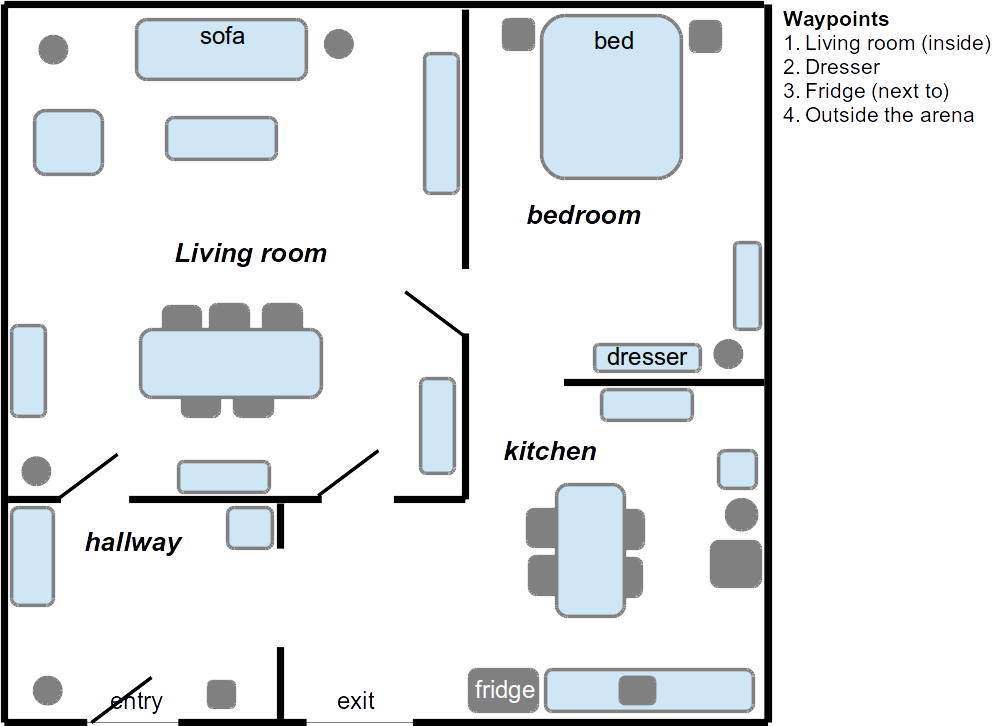
\includegraphics[width=0.5\columnwidth]{images/navigation.png}
	\caption{Navigation test: setup and execution example.}
	\label{fig:restaurant}
\end{figure}

\paragraph*{Remarks:}
\begin{enumerate}
	\item Depending on the layout of the arena, waypoint 1 and 2 may be swapped.
	\item Reaching a waypoint also includes the direction in which the robot should be looking when it reaches, which will be announced by the TC during the setup of the path.
	\item The distance between Waypoints 3 and 4 is about 10-20 meters.
\end{enumerate}

\subsection{Obstacles}
While navigating to waypoints 1, 2, and 3 the robot will find one of the following obstacles on its path:
\begin{itemize}
		\item \textbf{Small object:} Box sized object (between 5 and 15 cm per edge).  
		\item \textbf{3D Object:} A bar table, normal table, rolling chair: some object that is wider at its top than on its bottom, 
		  thus requiring more than just a laser scanner mounted near the ground to avoid obstacles.
		\item \textbf{Smart obstacle:} A person to whom the robot may speak to and kindly ask to move away. When interacting with people, the robot must look at the person and make clear is speaking with him/her.
	\end{itemize}

\subsection{Additional rules and remarks}
\begin{enumerate}
	\item \textbf{Waypoints:} Waypoints may be rooms, placement locations, furniture, beacons, landmarks, etc. The robot must clearly state when it has reached a waypoint or if it was not able to reach the waypoint.

	\item \textbf{Show must go on:} If a robot is unable to reach a waypoint, it must say it and proceed to the next one.

	\item \textbf{Closing internal doors:}  The internal door that will be shut will be the door on the route the robot has committed to. It will be shut right after the robot starts driving towards the door, but granting enough time to notice that the door is now closed.	

	\item \textbf{Moving objects:} If the robot finds on its way a \textit{static movable obstacle} (chair, cubes, toys, etc.) which is capable to move, it must announce is going to move an obstacle and then proceed to move the object apart with its manipulator, or by \textbf{gently} pushing it with its body.

	\item \textbf{Asking people to move away:} If the robot finds on its way a person blocking its path, it must announce it has found a person, \textit{gently} ask that person to move away and wait for the path to be clear. \textbf{Robots are not allowed to touch people}.

	\item \textbf{Following people:} 
	\begin{enumerate}
		\item \textbf{Instruction:} The robot interacts with the operator, \emph{not} the team. That is, the team is not allowed to instruct the operator.
		\item \textbf{Natural walking:} The operator has to walk \quotes{naturally}, i.e., move forward facing forward. 
		  The operator is not allowed to walk back, stand still, signal the robot or follow any re-calibration procedure.
		\item \textbf{Asking for passage:} The robot is allowed to (gently) ask people to step aside.
	\end{enumerate}
\end{enumerate}

\subsection{Data recording}
  Please record the following data (See \refsec{rule:datarecording}):
  \begin{itemize}
   \item Mapping data
   \item Plans
  \end{itemize}

\subsection{Referee instructions}

The referee needs to
\begin{itemize}
	\item Instruct the OC and volunteers on when and where locate objects.
	\item Instruct the OC and volunteers on when and which doors must be closed.
	\item Stop the robot immediately when it is about to collide.
\end{itemize}

\subsection{OC instructions}

\textbf{2 hours before the test}
\begin{itemize}
        \item Announce the entry and exit doors. 
	\item Announce the locations for waypoints 1, 2, and 3.
	\item Establish location for waypoint 4 and the path for the \textit{follow me} phase. 
\end{itemize}

\textbf{During the test}
\begin{itemize}
	\item Open and close the doors when instructed by the referee.
	\item Place the obstacles (or act as an obstacle) when instructed by the referee.
\end{itemize}

\newpage

\subsection{Score sheet}

The maximum time for this test is 5 minutes.

\begin{scorelist}

	\scoreheading{Waypoints}
	\scoreitem{10}{Reaching waypoint A}
	\scoreitem{10}{Reaching waypoint B}

	\scoreheading{Obstacles}
	\scoreitem{20}{Avoiding obstacle 1}
	\scoreitem{30}{Avoiding obstacle 2}
	\scoreitem{40}{Avoiding obstacle 3}
	\scoreitem{10}{Reporting unreachable waypoint due to an obstacle (will end the test)}

	\scoreheading{Doors}
	\scoreitem[2]{20}{Starting a new path after reaching a closed door}
	\scoreitem[2]{45}{Opening the door and continue instead of plan a new trajectory}

	\scoreheading{Optional tasks (up to 50 points)}
	\scoreitem{10}{Reaching waypoint}
	\scoreitem{40}{Reentering the arena after reach Waypoint 3}

	\setTotalScore{200}
\end{scorelist}


% Local Variables:
% TeX-master: "Rulebook"
% End:


% Local Variables:
% TeX-master: "Rulebook"
% End:
